% !TeX program = pdflatex
% Compiler Engineering Suite - shared standalone pdfLaTeX preamble
\documentclass[10pt,letterpaper]{article}
\usepackage[T1]{fontenc}
\usepackage[utf8]{inputenc}
\usepackage{lmodern}
\usepackage[margin=.78in,headheight=18pt]{geometry}
\usepackage[table]{xcolor}
\usepackage{microtype}
\usepackage{amsmath,amssymb}
\usepackage{booktabs,longtable,array}
\usepackage{enumitem}
\usepackage{fancyhdr}
\usepackage{hyperref}
\usepackage{needspace}
\usepackage{fancyvrb}
\usepackage{tikz}
\usetikzlibrary{arrows.meta,positioning,shapes.geometric}
\definecolor{CompilerBlue}{HTML}{1F4E79}
\definecolor{CompilerInk}{HTML}{263746}
\definecolor{CompilerGray}{HTML}{52616B}
\definecolor{CompilerLight}{HTML}{EFF4F8}
\hypersetup{colorlinks=true,linkcolor=CompilerBlue,urlcolor=CompilerBlue,citecolor=CompilerBlue}
\setlength{\parindent}{0pt}
\setlength{\parskip}{6pt plus 2pt}
\setlist[itemize]{leftmargin=*,itemsep=3pt,topsep=2pt}
\setlist[enumerate]{leftmargin=*,itemsep=3pt,topsep=2pt}
\pagestyle{fancy}
\fancyhf{}
\fancyhead[L]{\small\textcolor{CompilerGray}{Compiler Engineering Documentation Suite}}
\fancyhead[R]{\small\thepage}
\renewcommand{\headrulewidth}{.4pt}
\newcommand{\evidence}[1]{\par\smallskip\noindent\textbf{Evidence required:} #1\par}
\newcommand{\sourceanchor}[1]{\textbf{Book anchor:} #1\par}
\newcommand{\modern}{\textbf{Modern engineering extension (not attributed to the source book):} }
\newcommand{\writinglines}[1]{\par\noindent\rule{\linewidth}{.3pt}\par\vspace{#1\baselineskip}\noindent\rule{\linewidth}{.3pt}\par}
\newcommand{\checkboxline}[1]{\noindent $\square$\quad #1\par}
\newcommand{\formfield}[2]{\noindent\textbf{#1}\par\vspace{#2\baselineskip}\hrule\medskip}

\hypersetup{pdftitle={Compiler Engineering: 18-Week Curriculum},pdfauthor={Compiler Engineering Documentation Suite}}
\begin{document}
\begin{titlepage}
\centering\vspace*{1.0in}
{\Huge\bfseries\textcolor{CompilerBlue}{Compiler Engineering: 18-Week Curriculum}\par}
\vspace{.22in}{\Large Prerequisite graph, source reading and staged deliverables\par}
\vspace{.4in}{\large Compiler Engineering Documentation Suite\par}
\vfill
\begin{minipage}{.86\linewidth}\small
Source basis: Keith D. Cooper and Linda Torczon, \emph{Engineering a Compiler}, Third Edition (Morgan Kaufmann/Elsevier, 2023). All explanatory text, examples, questions, and implementation designs in this document are independently authored. The book is not included.\par\medskip
Document class: Curriculum.
\end{minipage}
\vfill\textcolor{CompilerGray}{Version 1.0 --- 2026-10-30}\par
\end{titlepage}
\tableofcontents\clearpage
\section{Prerequisite graph}
\textbf{Core prerequisites:} (A) programming in Python and C/C++; (B) discrete mathematics, sets, relations and proofs; (C) algorithms, asymptotic analysis and graph traversal; (D) computer architecture, registers and calling conventions; (E) version control and automated testing.
\begin{center}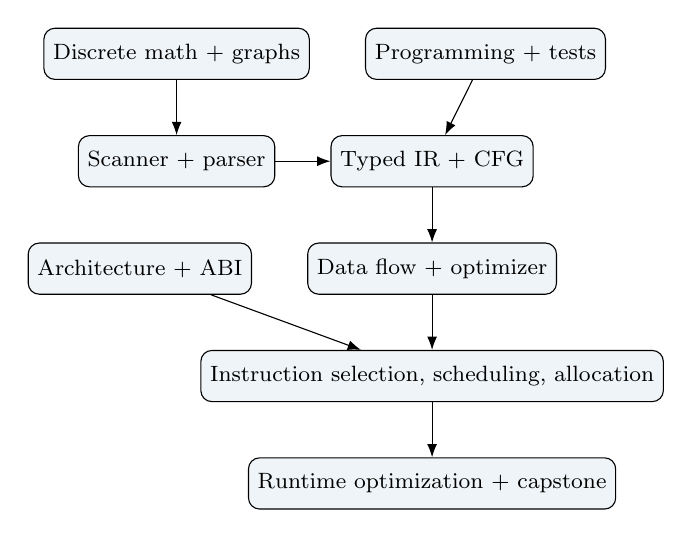
\begin{tikzpicture}[node distance=7mm and 7mm, every node/.style={draw,rounded corners,fill=CompilerLight,align=center,font=\footnotesize,minimum height=.65cm}]
\node (m) {Discrete math + graphs};\node[right=of m] (p) {Programming + tests};\node[below=of m] (l) {Scanner + parser};\node[right=of l] (ir) {Typed IR + CFG};\node[below=of ir] (df) {Data flow + optimizer};\node[left=of df] (hw) {Architecture + ABI};\node[below=of df] (be) {Instruction selection, scheduling, allocation};\node[below=of be] (jit) {Runtime optimization + capstone};
\draw[-{Latex}] (m)--(l);\draw[-{Latex}] (p)--(ir);\draw[-{Latex}] (l)--(ir);\draw[-{Latex}] (ir)--(df);\draw[-{Latex}] (hw)--(be);\draw[-{Latex}] (df)--(be);\draw[-{Latex}] (be)--(jit);
\end{tikzpicture}\end{center}

\section{Prerequisite-based 18-week plan}
\begin{longtable}{|p{0.16\linewidth}|p{0.13\linewidth}|p{0.15\linewidth}|p{0.27\linewidth}|p{0.22\linewidth}|}
\hline
Stage & Duration & Book chapters & Entry knowledge & Exit evidence\\ \hline\endfirsthead
\hline
Stage & Duration & Book chapters & Entry knowledge & Exit evidence\\ \hline\endhead
Foundation & Weeks 1--3 & 1,2,3 & Automata, grammars, induction, complexity, unit testing & Token and parse corpus, lexical/grammar invariants\\ \hline
Semantic front end & Weeks 4--6 & 4,5,6 & AST, symbol tables, storage, basic computer architecture & Typed AST, scope model and activation record ledger\\ \hline
Lowering and machine model & Weeks 7--8 & 7,11 & Address arithmetic, instruction encodings, calling convention & Guarded CFG and target instruction-selection model\\ \hline
Analysis and optimization & Weeks 9--12 & 8,9,10 & Set theory, graphs, fixed points, side-effect semantics & Liveness proof, safe optimization and differential test suite\\ \hline
Back end & Weeks 13--15 & 12,13 & Instruction latencies, interference graphs, register pressure & Schedule and spill-aware allocation trace\\ \hline
Runtime and capstone & Weeks 16--18 & 14 + all & AOT/JIT trade-offs, profiling and secure build & Measured end-to-end pipeline with threat model and release gate\\ \hline
\end{longtable}

\section{Reading and implementation protocol}
\begin{enumerate}
\item Read the book section and the corresponding standalone chapter guide; record exact section identifiers and definitions.
\item Perform the formal derivation by hand before implementation.
\item Write a test oracle and negative corpus before optimization.
\item Implement, test and review changes; run sanitizer builds when applicable.
\item Capture cost model, benchmark controls and evidence sheet.
\item Gate progression on the competency matrix; prerequisites are skills, not elapsed time.
\end{enumerate}

\section{Completion standards}
\begin{longtable}{|p{0.22\linewidth}|p{0.71\linewidth}|}
\hline
Track & Required demonstration\\ \hline\endfirsthead
\hline
Track & Required demonstration\\ \hline\endhead
Foundation & Reproducible lexical and syntactic acceptance tests\\ \hline
Intermediate & Typed IR printer, CFG consistency and loop/control translation\\ \hline
Advanced & Fixed-point liveness, safe rewrites and backend legality\\ \hline
Capstone & End-to-end traceability, threat model, multi-language tests, repeatable measurements\\ \hline
\end{longtable}


\end{document}
